%%%%%%%%%%%%%%%%%%%%%%%%%%%%%%%%%%%%%%%%%
% The Legrand Orange Book
% LaTeX Template
% Version 2.3 (8/8/17)
%
% This template has been downloaded from:
% http://www.LaTeXTemplates.com
%
% Original author:
% Mathias Legrand (legrand.mathias@gmail.com) with modifications by:
% Vel (vel@latextemplates.com)
%
% License:
% CC BY-NC-SA 3.0 (http://creativecommons.org/licenses/by-nc-sa/3.0/)
%
% Compiling this template:
% This template uses biber for its bibliography and makeindex for its index.
% When you first open the template, compile it from the command line with the 
% commands below to make sure your LaTeX distribution is configured correctly:
%
% 1) pdflatex main
% 2) makeindex main.idx -s StyleInd.ist
% 3) biber main
% 4) pdflatex main x 2
%
% After this, when you wish to update the bibliography/index use the appropriate
% command above and make sure to compile with pdflatex several times 
% afterwards to propagate your changes to the document.
%
% This template also uses a number of packages which may need to be
% updated to the newest versions for the template to compile. It is strongly
% recommended you update your LaTeX distribution if you have any
% compilation errors.
%
% Important note:
% Chapter heading images should have a 2:1 width:height ratio,
% e.g. 920px width and 460px height.
%
%%%%%%%%%%%%%%%%%%%%%%%%%%%%%%%%%%%%%%%%%

%----------------------------------------------------------------------------------------
%	PACKAGES AND OTHER DOCUMENT CONFIGURATIONS
%----------------------------------------------------------------------------------------

\documentclass[11pt,fleqn]{book} % Default font size and left-justified equations

%----------------------------------------------------------------------------------------

%%%%%%%%%%%%%%%%%%%%%%%%%%%%%%%%%%%%%%%%%
% The Legrand Orange Book
% Structural Definitions File
% Version 2.0 (9/2/15)
%
% Original author:
% Mathias Legrand (legrand.mathias@gmail.com) with modifications by:
% Vel (vel@latextemplates.com)
% 
% This file has been downloaded from:
% http://www.LaTeXTemplates.com
%
% License:
% CC BY-NC-SA 3.0 (http://creativecommons.org/licenses/by-nc-sa/3.0/)
%
%%%%%%%%%%%%%%%%%%%%%%%%%%%%%%%%%%%%%%%%%

%----------------------------------------------------------------------------------------
%	VARIOUS REQUIRED PACKAGES AND CONFIGURATIONS
%----------------------------------------------------------------------------------------

\usepackage[top=3cm,bottom=3cm,left=3cm,right=3cm,headsep=10pt,letterpaper]{geometry} % Page margins

\usepackage{graphicx} % Required for including pictures
\graphicspath{{Pictures/}} % Specifies the directory where pictures are stored

%\usepackage{lipsum} % Inserts dummy text

\usepackage{tikz} % Required for drawing custom shapes

\usepackage[spanish,mexico]{babel}
%\usepackage[english]{babel} % English language/hyphenation


\usepackage{colortbl} 
\usepackage{float}
\usepackage{enumerate}

\usepackage[shortlabels]{enumitem} % Customize lists
\setlist{nolistsep} % Reduce spacing between bullet points and numbered lists

\usepackage{booktabs} % Required for nicer horizontal rules in tables

\usepackage{xcolor} % Required for specifying colors by name
\definecolor{ocre}{RGB}{243,102,25} % Define the orange color used for highlighting throughout the book

%----------------------------------------------------------------------------------------
%	FONTS
%----------------------------------------------------------------------------------------

\usepackage{avant} % Use the Avantgarde font for headings
%\usepackage{times} % Use the Times font for headings
\usepackage{mathptmx} % Use the Adobe Times Roman as the default text font together with math symbols from the Sym­bol, Chancery and Com­puter Modern fonts

\usepackage{microtype} % Slightly tweak font spacing for aesthetics
\usepackage[utf8]{inputenc} % Required for including letters with accents
\usepackage[T1]{fontenc} % Use 8-bit encoding that has 256 glyphs

%----------------------------------------------------------------------------------------
%	BIBLIOGRAPHY AND INDEX
%----------------------------------------------------------------------------------------

\usepackage[style=numeric,citestyle=numeric,sorting=nyt,sortcites=true,autopunct=true,babel=hyphen,hyperref=true,abbreviate=false,backref=true,backend=biber]{biblatex}
\addbibresource{bibliography.bib} % BibTeX bibliography file
\defbibheading{bibempty}{}

\usepackage{calc} % For simpler calculation - used for spacing the index letter headings correctly
\usepackage{makeidx} % Required to make an index
\makeindex % Tells LaTeX to create the files required for indexing

%----------------------------------------------------------------------------------------
%	MAIN TABLE OF CONTENTS
%----------------------------------------------------------------------------------------

\usepackage{titletoc} % Required for manipulating the table of contents

\contentsmargin{0cm} % Removes the default margin

% Part text styling
\titlecontents{part}[0cm]
{\addvspace{20pt}\centering\large\bfseries}
{}
{}
{}

% Chapter text styling
\titlecontents{chapter}[1.25cm] % Indentation
{\addvspace{12pt}\large\sffamily\bfseries} % Spacing and font options for chapters
{\color{ocre!60}\contentslabel[\Large\thecontentslabel]{1.25cm}\color{ocre}} % Chapter number
{\color{ocre}}  
{\color{ocre!60}\normalsize\;\titlerule*[.5pc]{.}\;\thecontentspage} % Page number

% Section text styling
\titlecontents{section}[1.25cm] % Indentation
{\addvspace{3pt}\sffamily\bfseries} % Spacing and font options for sections
{\contentslabel[\thecontentslabel]{1.25cm}} % Section number
{}
{\hfill\color{black}\thecontentspage} % Page number
[]

% Subsection text styling
\titlecontents{subsection}[1.25cm] % Indentation
{\addvspace{1pt}\sffamily\small} % Spacing and font options for subsections
{\contentslabel[\thecontentslabel]{1.25cm}} % Subsection number
{}
{\ \titlerule*[.5pc]{.}\;\thecontentspage} % Page number
[]

% List of figures
\titlecontents{figure}[0em]
{\addvspace{-5pt}\sffamily}
{\thecontentslabel\hspace*{1em}}
{}
{\ \titlerule*[.5pc]{.}\;\thecontentspage}
[]

% List of tables
\titlecontents{table}[0em]
{\addvspace{-5pt}\sffamily}
{\thecontentslabel\hspace*{1em}}
{}
{\ \titlerule*[.5pc]{.}\;\thecontentspage}
[]

%----------------------------------------------------------------------------------------
%	MINI TABLE OF CONTENTS IN PART HEADS
%----------------------------------------------------------------------------------------

% Chapter text styling
\titlecontents{lchapter}[0em] % Indenting
{\addvspace{15pt}\large\sffamily\bfseries} % Spacing and font options for chapters
{\color{ocre}\contentslabel[\Large\thecontentslabel]{1.25cm}\color{ocre}} % Chapter number
{}  
{\color{ocre}\normalsize\sffamily\bfseries\;\titlerule*[.5pc]{.}\;\thecontentspage} % Page number

% Section text styling
\titlecontents{lsection}[0em] % Indenting
{\sffamily\small} % Spacing and font options for sections
{\contentslabel[\thecontentslabel]{1.25cm}} % Section number
{}
{}

% Subsection text styling
\titlecontents{lsubsection}[.5em] % Indentation
{\normalfont\footnotesize\sffamily} % Font settings
{}
{}
{}

%----------------------------------------------------------------------------------------
%	PAGE HEADERS
%----------------------------------------------------------------------------------------

\usepackage{fancyhdr} % Required for header and footer configuration

\pagestyle{fancy}
\renewcommand{\chaptermark}[1]{\markboth{\sffamily\normalsize\bfseries\chaptername\ \thechapter.\ #1}{}} % Chapter text font settings
\renewcommand{\sectionmark}[1]{\markright{\sffamily\normalsize\thesection\hspace{5pt}#1}{}} % Section text font settings
\fancyhf{} \fancyhead[LE,RO]{\sffamily\normalsize\thepage} % Font setting for the page number in the header
\fancyhead[LO]{\rightmark} % Print the nearest section name on the left side of odd pages
\fancyhead[RE]{\leftmark} % Print the current chapter name on the right side of even pages
\renewcommand{\headrulewidth}{0.5pt} % Width of the rule under the header
\addtolength{\headheight}{2.5pt} % Increase the spacing around the header slightly
\renewcommand{\footrulewidth}{0pt} % Removes the rule in the footer
\fancypagestyle{plain}{\fancyhead{}\renewcommand{\headrulewidth}{0pt}} % Style for when a plain pagestyle is specified

% Removes the header from odd empty pages at the end of chapters
\makeatletter
\renewcommand{\cleardoublepage}{
\clearpage\ifodd\c@page\else
\hbox{}
\vspace*{\fill}
\thispagestyle{empty}
\newpage
\fi}

%----------------------------------------------------------------------------------------
%	THEOREM STYLES
%----------------------------------------------------------------------------------------

\usepackage{amsmath,amsfonts,amssymb,amsthm} % For math equations, theorems, symbols, etc

\newcommand{\intoo}[2]{\mathopen{]}#1\,;#2\mathclose{[}}
\newcommand{\ud}{\mathop{\mathrm{{}d}}\mathopen{}}
\newcommand{\intff}[2]{\mathopen{[}#1\,;#2\mathclose{]}}
\newtheorem{notation}{Notation}[chapter]

% Boxed/framed environments
\newtheoremstyle{ocrenumbox}% % Theorem style name
{0pt}% Space above
{0pt}% Space below
{\normalfont}% % Body font
{}% Indent amount
{\small\bf\sffamily\color{ocre}}% % Theorem head font
{\;}% Punctuation after theorem head
{0.25em}% Space after theorem head
{\small\sffamily\color{ocre}\thmname{#1}\nobreakspace\thmnumber{\@ifnotempty{#1}{}\@upn{#2}}% Theorem text (e.g. Theorem 2.1)
\thmnote{\nobreakspace\the\thm@notefont\sffamily\bfseries\color{black}---\nobreakspace#3.}} % Optional theorem note
\renewcommand{\qedsymbol}{$\blacksquare$}% Optional qed square

\newtheoremstyle{blacknumex}% Theorem style name
{5pt}% Space above
{5pt}% Space below
{\normalfont}% Body font
{} % Indent amount
{\small\bf\sffamily}% Theorem head font
{\;}% Punctuation after theorem head
{0.25em}% Space after theorem head
{\small\sffamily{\tiny\ensuremath{\blacksquare}}\nobreakspace\thmname{#1}\nobreakspace\thmnumber{\@ifnotempty{#1}{}\@upn{#2}}% Theorem text (e.g. Theorem 2.1)
\thmnote{\nobreakspace\the\thm@notefont\sffamily\bfseries---\nobreakspace#3.}}% Optional theorem note

\newtheoremstyle{blacknumbox} % Theorem style name
{0pt}% Space above
{0pt}% Space below
{\normalfont}% Body font
{}% Indent amount
{\small\bf\sffamily}% Theorem head font
{\;}% Punctuation after theorem head
{0.25em}% Space after theorem head
{\small\sffamily\thmname{#1}\nobreakspace\thmnumber{\@ifnotempty{#1}{}\@upn{#2}}% Theorem text (e.g. Theorem 2.1)
\thmnote{\nobreakspace\the\thm@notefont\sffamily\bfseries---\nobreakspace#3.}}% Optional theorem note

% Non-boxed/non-framed environments
\newtheoremstyle{ocrenum}% % Theorem style name
{5pt}% Space above
{5pt}% Space below
{\normalfont}% % Body font
{}% Indent amount
{\small\bf\sffamily\color{ocre}}% % Theorem head font
{\;}% Punctuation after theorem head
{0.25em}% Space after theorem head
{\small\sffamily\color{ocre}\thmname{#1}\nobreakspace\thmnumber{\@ifnotempty{#1}{}\@upn{#2}}% Theorem text (e.g. Theorem 2.1)
\thmnote{\nobreakspace\the\thm@notefont\sffamily\bfseries\color{black}---\nobreakspace#3.}} % Optional theorem note
\renewcommand{\qedsymbol}{$\blacksquare$}% Optional qed square
\makeatother

% Defines the theorem text style for each type of theorem to one of the three styles above
\newcounter{dummy} 
\numberwithin{dummy}{section}
\theoremstyle{ocrenumbox}
\newtheorem{theoremeT}[dummy]{Teorema}
\newtheorem{problem}{Problema}[chapter]
\newtheorem{exerciseT}{Ejercicio}[chapter]
\theoremstyle{blacknumex}
\newtheorem{exampleT}{Ejemplo}[chapter]
\theoremstyle{blacknumbox}
\newtheorem{vocabulary}{Vocabulario}[chapter]
\newtheorem{definitionT}{Definición}[section]
\newtheorem{corollaryT}[dummy]{Corollary}
\theoremstyle{ocrenum}
\newtheorem{proposition}[dummy]{Proposición}

%----------------------------------------------------------------------------------------
%	DEFINITION OF COLORED BOXES
%----------------------------------------------------------------------------------------

\RequirePackage[framemethod=default]{mdframed} % Required for creating the theorem, definition, exercise and corollary boxes

% Theorem box
\newmdenv[skipabove=7pt,
skipbelow=7pt,
backgroundcolor=black!5,
linecolor=ocre,
innerleftmargin=5pt,
innerrightmargin=5pt,
innertopmargin=5pt,
leftmargin=0cm,
rightmargin=0cm,
innerbottommargin=5pt]{tBox}

% Exercise box	  
\newmdenv[skipabove=7pt,
skipbelow=7pt,
rightline=false,
leftline=true,
topline=false,
bottomline=false,
backgroundcolor=ocre!10,
linecolor=ocre,
innerleftmargin=5pt,
innerrightmargin=5pt,
innertopmargin=5pt,
innerbottommargin=5pt,
leftmargin=0cm,
rightmargin=0cm,
linewidth=4pt]{eBox}	

% Definition box
\newmdenv[skipabove=7pt,
skipbelow=7pt,
rightline=false,
leftline=true,
topline=false,
bottomline=false,
linecolor=ocre,
innerleftmargin=5pt,
innerrightmargin=5pt,
innertopmargin=0pt,
leftmargin=0cm,
rightmargin=0cm,
linewidth=4pt,
innerbottommargin=0pt]{dBox}	

% Corollary box
\newmdenv[skipabove=7pt,
skipbelow=7pt,
rightline=false,
leftline=true,
topline=false,
bottomline=false,
linecolor=gray,
backgroundcolor=black!5,
innerleftmargin=5pt,
innerrightmargin=5pt,
innertopmargin=5pt,
leftmargin=0cm,
rightmargin=0cm,
linewidth=4pt,
innerbottommargin=5pt]{cBox}

% Creates an environment for each type of theorem and assigns it a theorem text style from the "Theorem Styles" section above and a colored box from above
\newenvironment{theorem}{\begin{tBox}\begin{theoremeT}}{\end{theoremeT}\end{tBox}}
\newenvironment{exercise}{\begin{eBox}\begin{exerciseT}}{\hfill{\color{ocre}\tiny\ensuremath{\blacksquare}}\end{exerciseT}\end{eBox}}				  
\newenvironment{definition}{\begin{dBox}\begin{definitionT}}{\end{definitionT}\end{dBox}}	
\newenvironment{example}{\begin{exampleT}}{\hfill{\tiny\ensuremath{\blacksquare}}\end{exampleT}}		
\newenvironment{corollary}{\begin{cBox}\begin{corollaryT}}{\end{corollaryT}\end{cBox}}	

%----------------------------------------------------------------------------------------
%	REMARK ENVIRONMENT
%----------------------------------------------------------------------------------------

\newenvironment{remark}{\par\vspace{10pt}\small % Vertical white space above the remark and smaller font size
\begin{list}{}{
\leftmargin=35pt % Indentation on the left
\rightmargin=25pt}\item\ignorespaces % Indentation on the right
\makebox[-2.5pt]{\begin{tikzpicture}[overlay]
\node[draw=ocre!60,line width=1pt,circle,fill=ocre!25,font=\sffamily\bfseries,inner sep=2pt,outer sep=0pt] at (-15pt,0pt){\textcolor{ocre}{R}};\end{tikzpicture}} % Orange R in a circle
\advance\baselineskip -1pt}{\end{list}\vskip5pt} % Tighter line spacing and white space after remark

%----------------------------------------------------------------------------------------
%	SECTION NUMBERING IN THE MARGIN
%----------------------------------------------------------------------------------------

\makeatletter
\renewcommand{\@seccntformat}[1]{\llap{\textcolor{ocre}{\csname the#1\endcsname}\hspace{1em}}}                    
\renewcommand{\section}{\@startsection{section}{1}{\z@}
{-4ex \@plus -1ex \@minus -.4ex}
{1ex \@plus.2ex }
{\normalfont\large\sffamily\bfseries}}
\renewcommand{\subsection}{\@startsection {subsection}{2}{\z@}
{-3ex \@plus -0.1ex \@minus -.4ex}
{0.5ex \@plus.2ex }
{\normalfont\sffamily\bfseries}}
\renewcommand{\subsubsection}{\@startsection {subsubsection}{3}{\z@}
{-2ex \@plus -0.1ex \@minus -.2ex}
{.2ex \@plus.2ex }
{\normalfont\small\sffamily\bfseries}}                        
\renewcommand\paragraph{\@startsection{paragraph}{4}{\z@}
{-2ex \@plus-.2ex \@minus .2ex}
{.1ex}
{\normalfont\small\sffamily\bfseries}}

%----------------------------------------------------------------------------------------
%	PART HEADINGS
%----------------------------------------------------------------------------------------

% numbered part in the table of contents
\newcommand{\@mypartnumtocformat}[2]{%
\setlength\fboxsep{0pt}%
\noindent\colorbox{ocre!20}{\strut\parbox[c][.7cm]{\ecart}{\color{ocre!70}\Large\sffamily\bfseries\centering#1}}\hskip\esp\colorbox{ocre!40}{\strut\parbox[c][.7cm]{\linewidth-\ecart-\esp}{\Large\sffamily\centering#2}}}%
%%%%%%%%%%%%%%%%%%%%%%%%%%%%%%%%%%
% unnumbered part in the table of contents
\newcommand{\@myparttocformat}[1]{%
\setlength\fboxsep{0pt}%
\noindent\colorbox{ocre!40}{\strut\parbox[c][.7cm]{\linewidth}{\Large\sffamily\centering#1}}}%
%%%%%%%%%%%%%%%%%%%%%%%%%%%%%%%%%%
\newlength\esp
\setlength\esp{4pt}
\newlength\ecart
\setlength\ecart{1.2cm-\esp}
\newcommand{\thepartimage}{}%
\newcommand{\partimage}[1]{\renewcommand{\thepartimage}{#1}}%
\def\@part[#1]#2{%
\ifnum \c@secnumdepth >-2\relax%
\refstepcounter{part}%
\addcontentsline{toc}{part}{\texorpdfstring{\protect\@mypartnumtocformat{\thepart}{#1}}{\partname~\thepart\ ---\ #1}}
\else%
\addcontentsline{toc}{part}{\texorpdfstring{\protect\@myparttocformat{#1}}{#1}}%
\fi%
\startcontents%
\markboth{}{}%
{\thispagestyle{empty}%
\begin{tikzpicture}[remember picture,overlay]%
\node at (current page.north west){\begin{tikzpicture}[remember picture,overlay]%	
\fill[ocre!20](0cm,0cm) rectangle (\paperwidth,-\paperheight);
\node[anchor=north] at (4cm,-3.25cm){\color{ocre!40}\fontsize{220}{100}\sffamily\bfseries\thepart}; 
\node[anchor=south east] at (\paperwidth-1cm,-\paperheight+1cm){\parbox[t][][t]{8.5cm}{
\printcontents{l}{0}{\setcounter{tocdepth}{1}}%
}};
\node[anchor=north east] at (\paperwidth-1.5cm,-3.25cm){\parbox[t][][t]{15cm}{\strut\raggedleft\color{white}\fontsize{30}{30}\sffamily\bfseries#2}};
\end{tikzpicture}};
\end{tikzpicture}}%
\@endpart}
\def\@spart#1{%
\startcontents%
\phantomsection
{\thispagestyle{empty}%
\begin{tikzpicture}[remember picture,overlay]%
\node at (current page.north west){\begin{tikzpicture}[remember picture,overlay]%	
\fill[ocre!20](0cm,0cm) rectangle (\paperwidth,-\paperheight);
\node[anchor=north east] at (\paperwidth-1.5cm,-3.25cm){\parbox[t][][t]{15cm}{\strut\raggedleft\color{white}\fontsize{30}{30}\sffamily\bfseries#1}};
\end{tikzpicture}};
\end{tikzpicture}}
\addcontentsline{toc}{part}{\texorpdfstring{%
\setlength\fboxsep{0pt}%
\noindent\protect\colorbox{ocre!40}{\strut\protect\parbox[c][.7cm]{\linewidth}{\Large\sffamily\protect\centering #1\quad\mbox{}}}}{#1}}%
\@endpart}
\def\@endpart{\vfil\newpage
\if@twoside
\if@openright
\null
\thispagestyle{empty}%
\newpage
\fi
\fi
\if@tempswa
\twocolumn
\fi}

%----------------------------------------------------------------------------------------
%	CHAPTER HEADINGS
%----------------------------------------------------------------------------------------

% A switch to conditionally include a picture, implemented by  Christian Hupfer
\newif\ifusechapterimage
\usechapterimagetrue
\newcommand{\thechapterimage}{}%
\newcommand{\chapterimage}[1]{\ifusechapterimage\renewcommand{\thechapterimage}{#1}\fi}%
\newcommand{\autodot}{.}
\def\@makechapterhead#1{%
{\parindent \z@ \raggedright \normalfont
\ifnum \c@secnumdepth >\m@ne
\if@mainmatter
\begin{tikzpicture}[remember picture,overlay]
\node at (current page.north west)
{\begin{tikzpicture}[remember picture,overlay]
\node[anchor=north west,inner sep=0pt] at (0,0) {\ifusechapterimage\includegraphics[width=\paperwidth]{\thechapterimage}\fi};
\draw[anchor=west] (\Gm@lmargin,-9cm) node [line width=2pt,rounded corners=15pt,draw=ocre,fill=white,fill opacity=0.5,inner sep=15pt]{\strut\makebox[22cm]{}};
\draw[anchor=west] (\Gm@lmargin+.3cm,-9cm) node {\huge\sffamily\bfseries\color{black}\thechapter\autodot~#1\strut};
\end{tikzpicture}};
\end{tikzpicture}
\else
\begin{tikzpicture}[remember picture,overlay]
\node at (current page.north west)
{\begin{tikzpicture}[remember picture,overlay]
\node[anchor=north west,inner sep=0pt] at (0,0) {\ifusechapterimage\includegraphics[width=\paperwidth]{\thechapterimage}\fi};
\draw[anchor=west] (\Gm@lmargin,-9cm) node [line width=2pt,rounded corners=15pt,draw=ocre,fill=white,fill opacity=0.5,inner sep=15pt]{\strut\makebox[22cm]{}};
\draw[anchor=west] (\Gm@lmargin+.3cm,-9cm) node {\huge\sffamily\bfseries\color{black}#1\strut};
\end{tikzpicture}};
\end{tikzpicture}
\fi\fi\par\vspace*{270\p@}}}

%-------------------------------------------

\def\@makeschapterhead#1{%
\begin{tikzpicture}[remember picture,overlay]
\node at (current page.north west)
{\begin{tikzpicture}[remember picture,overlay]
\node[anchor=north west,inner sep=0pt] at (0,0) {\ifusechapterimage\includegraphics[width=\paperwidth]{\thechapterimage}\fi};
\draw[anchor=west] (\Gm@lmargin,-9cm) node [line width=2pt,rounded corners=15pt,draw=ocre,fill=white,fill opacity=0.5,inner sep=15pt]{\strut\makebox[22cm]{}};
\draw[anchor=west] (\Gm@lmargin+.3cm,-9cm) node {\huge\sffamily\bfseries\color{black}#1\strut};
\end{tikzpicture}};
\end{tikzpicture}
\par\vspace*{270\p@}}
\makeatother

%----------------------------------------------------------------------------------------
%	HYPERLINKS IN THE DOCUMENTS
%----------------------------------------------------------------------------------------

\usepackage{hyperref}
\hypersetup{hidelinks,backref=true,pagebackref=true,hyperindex=true,colorlinks=false,breaklinks=true,urlcolor= ocre,bookmarks=true,bookmarksopen=false,pdftitle={Metodos Numericos},pdfauthor={Hector Selley}}
\usepackage{bookmark}
\bookmarksetup{
open,
numbered,
addtohook={%
\ifnum\bookmarkget{level}=0 % chapter
\bookmarksetup{bold}%
\fi
\ifnum\bookmarkget{level}=-1 % part
\bookmarksetup{color=ocre,bold}%
\fi
}
}
\usepackage{rotating}
\usepackage[
ruled,
vlined,
%commentsnumbered,
linesnumbered
%,algosection
,spanish
]{algorithm2e}
\usepackage{multicol} % Insert the commands.tex file which contains the majority of the structure behind the template

\begin{document}

%----------------------------------------------------------------------------------------
%	TITLE PAGE
%----------------------------------------------------------------------------------------

\begingroup
\thispagestyle{empty}
\begin{tikzpicture}[remember picture,overlay]
\node[inner sep=0pt] (background) at (current page.center) {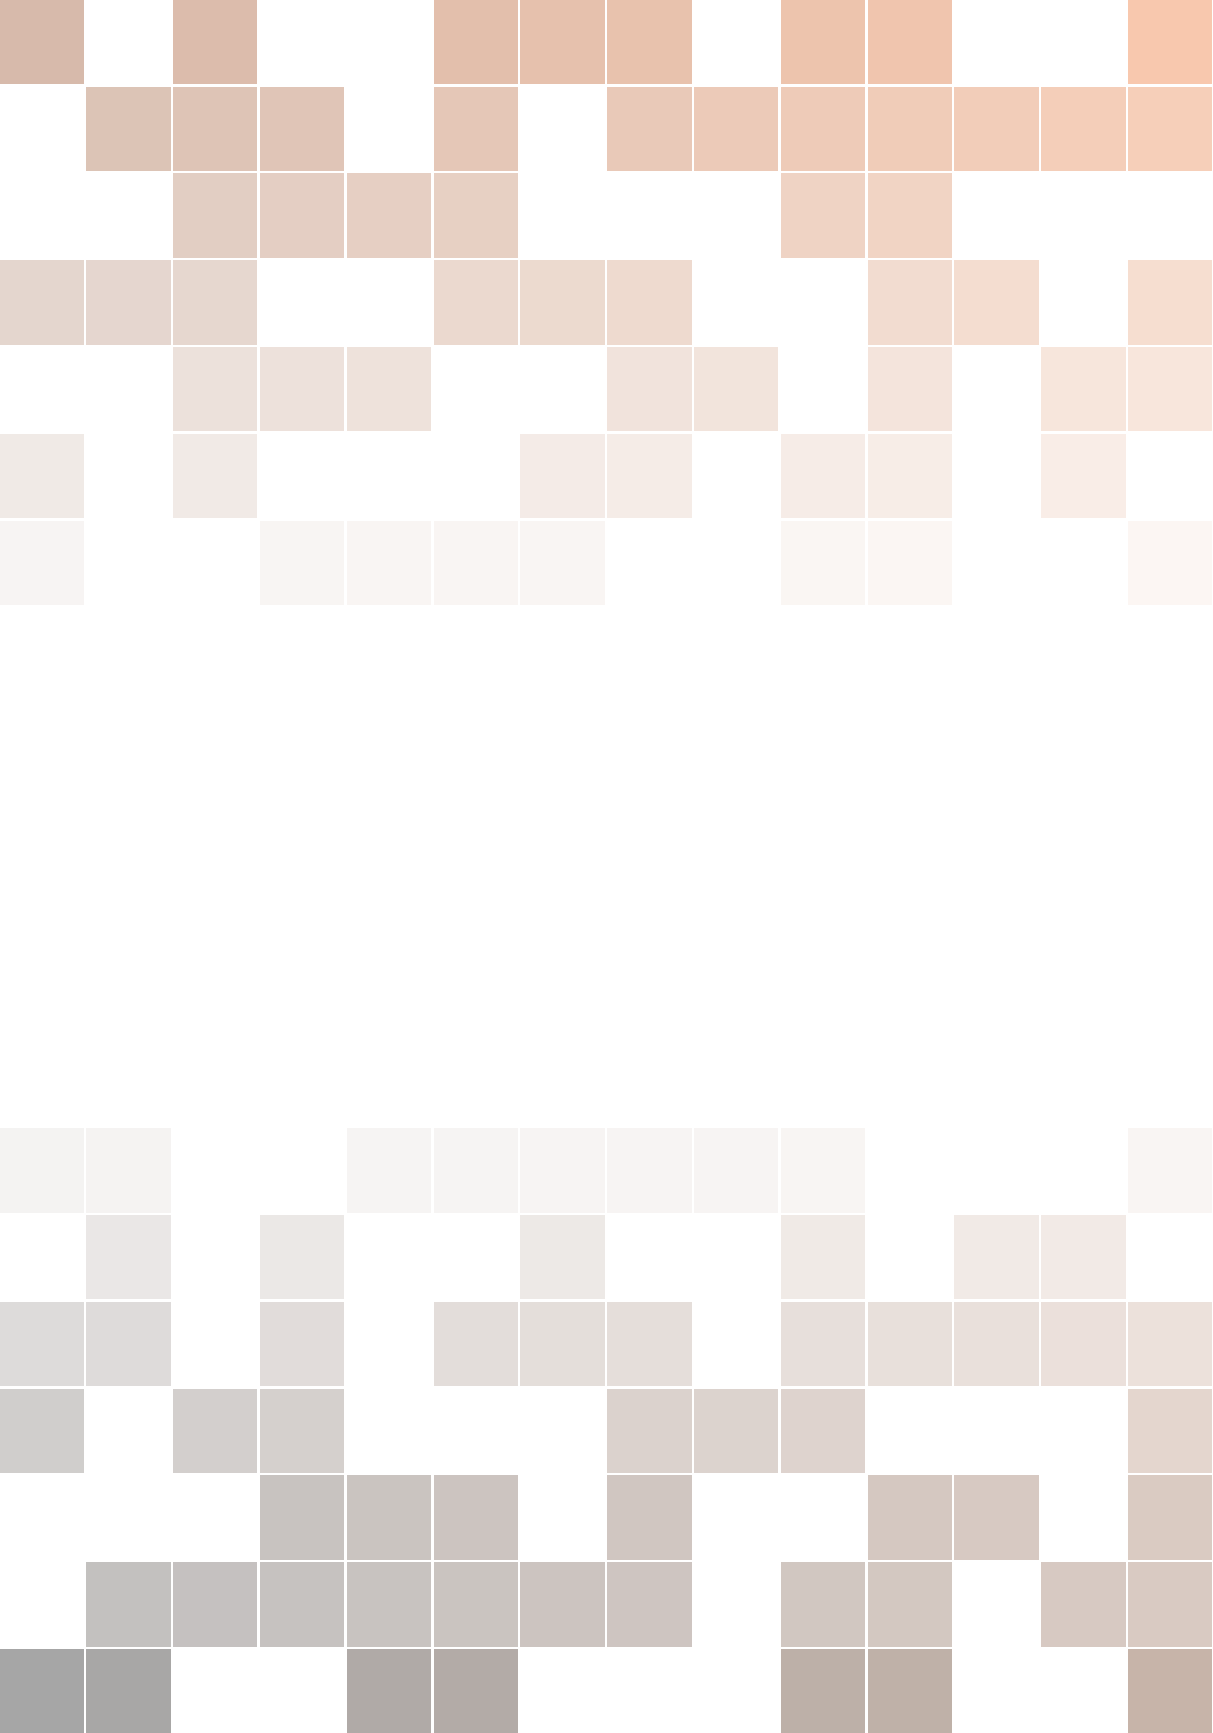
\includegraphics[width=\paperwidth]{background}};
\draw (current page.center) node [fill=ocre!30!white,fill opacity=0.6,text opacity=1,inner sep=1cm]{\Huge\centering\bfseries\sffamily\parbox[c][][t]{\paperwidth}
{\centering Métodos Numéricos\\[15pt] % Book title
{\Large Facultad de Ingeniería - Universidad Anáhuac}\\[20pt] % Subtitle
{\huge Dr. Héctor Selley}}}; % Author name
\end{tikzpicture}
\vfill
\endgroup

%----------------------------------------------------------------------------------------
%	COPYRIGHT PAGE
%----------------------------------------------------------------------------------------

%\newpage
%~\vfill
%\thispagestyle{empty}
%
%\noindent Copyright \copyright\ 2013 John Smith\\ % Copyright notice
%
%\noindent \textsc{Published by Publisher}\\ % Publisher
%
%\noindent \textsc{book-website.com}\\ % URL
%
%\noindent Licensed under the Creative Commons Attribution-NonCommercial 3.0 Unported License (the ``License''). You may not use this file except in compliance with the License. You may obtain a copy of the License at \url{http://creativecommons.org/licenses/by-nc/3.0}. Unless required by applicable law or agreed to in writing, software distributed under the License is distributed on an \textsc{``as is'' basis, without warranties or conditions of any kind}, either express or implied. See the License for the specific language governing permissions and limitations under the License.\\ % License information
%
%\noindent \textit{First printing, March 2013} % Printing/edition date

%----------------------------------------------------------------------------------------
%	TABLE OF CONTENTS
%----------------------------------------------------------------------------------------

\usechapterimagefalse % If you don't want to include a chapter image, use this to toggle images off - it can be enabled later with \usechapterimagetrue
%\usechapterimagetrue

\chapterimage{chapter_head_1.pdf} % Table of contents heading image

\pagestyle{empty} % No headers

\tableofcontents % Print the table of contents itself

\cleardoublepage % Forces the first chapter to start on an odd page so it's on the right

\pagestyle{fancy} % Print headers again

%----------------------------------------------------------------------------------------
%	INDEX
%----------------------------------------------------------------------------------------

\cleardoublepage
\phantomsection
\setlength{\columnsep}{0.75cm}
\addcontentsline{toc}{chapter}{\textcolor{ocre}{Index}}
\printindex

%----------------------------------------------------------------------------------------

%----------------------------------------------------------------------------------------
%	PART
%----------------------------------------------------------------------------------------

%\part{Parte 1}

%----------------------------------------------------------------------------------------
%	CHAPTER 1
%----------------------------------------------------------------------------------------

\chapterimage{chapter_head_2.pdf} % Chapter heading image

\chapter{Introducción}

\section{Panorama histórico}

\section{Sistemas de numeración}

Numéricamente los errores de redondeo se relacionan de manera directa con la forma en que se guardan los números en la memoria de la computadora. 
La unidad fundamental mediante la cual se representa la información se llama \textit{término}. Ésta es una entidad que consiste en una cadena de 
\textit{dígitos binarios} o \textit{bits}. Generalmente, los números son guardados en uno más términos. Para entender cómo se realiza esto, 
estudiaremos los sistemas numéricos.

\begin{center}
  \textit{“Solo existen 10 tipos de personas, las que entienden el binario y las que no”} 
\end{center}
Un sistema de numeración es un conjunto de símbolos y reglas que permiten construir todos los números válidos. Los sistemas de numeración más comunes son el decimal (base 10), 
binario (base 2), octal (base 8) y hexadecimal (base 16).\\
Un número decimal tal como 7392 representa una cantidad igual a 7 unidades de mil, más 3 centenas, más 9 decenas, más 2 unidades. Las unidades de mil, centenas, etc., son potencias 
de 10 implícitamente indicadas por la posición de los coeficientes. Esto es:
$$7 \times 10^{3} + 3 \times 10^{2} + 9 \times 10^{1} + 2 \times 10^{0} = 7000 + 300 + 90 + 2 = 7392$$
Y para el caso del número no entero $654.32$:
$$6 \times 10^{2} + 5 \times 10^{1} + 4 \times 10^{0} + 3 \times 10^{-1}+ 2 \times 10^{-2} = 600 + 50 + 4 + 0.3 + 0.02 = 654.32$$
Se dice que el sistema de números decimales tiene base 10 debido a que usan diez dígitos, los números del 0 al 9, y que los coeficientes son multiplicados por potencias de 10. 
Por otro lado, el sistema de numeración binario sólo tiene dos elementos: 0 y 1. Por ejemplo, el equivalente decimal del número binario 11010.11 es 26.75 como se demuestra en la 
multiplicación de los coeficientes por potencias de 2:
$$1 \times 2^{4} + 1 \times 2^{3} + 0 \times 2^{2} + 1 \times 2^{1} + 0 \times 2^{0} + 1 \times 2^{-1} + 1 \times 2^{-2} = 26.75$$
Para distinguir los números con bases diferentes, se encierran los coeficientes entre paréntesis y se escribe un suscrito igual a la base usada. Un ejemplo de una base 5 sería:
$$(4021.2)_{5} = 4 \times 5^{3} + 0 \times 5^{2} + 2 \times 5^{1} + 1 \times 5^{0} + 2 \times 5^{-1} = (511.4)_{10}$$
Nótese que los únicos valores posibles para los coeficientes de base 5 pueden ser 0, 1, 2, 3 y 4.\\
En el sistema de numeración hexadecimal (base 16) se presentan los primeros diez dígitos del sistema decimal y las letras A, B, C, D, E y F para representar los números 
10, 11, 12, 13, 14 y 15. Por ejemplo, dado el número hexadecimal se obtiene su equivalente en decimal:
$$(B65F)_{16} = 11 \times 16^{3} + 6 \times 16^{2} + 5 \times 16^{1} + 15 \times 16^{0} = (46687)_{10}$$
En la Tabla \ref{table:sistemasNumeracion} se muestran los primeros 16 números en los sistemas decimal, binario, octal y hexadecimal.

  \begin{table}[ht]
	\centering	
	\begin{tabular}{c c c c}
	  \toprule
	  \textbf{Decimal (Base 10)} & \textbf{Binario (Base 2)} & \textbf{Octal (Base 8)} & \textbf{Hexadecimal (Base 16)} \\
	  \midrule
	  00 & 0000 & 00 & 0\\
	  01 & 0001 & 01 & 1\\
	  02 & 0010 & 02 & 2\\
	  03 & 0011 & 03 & 3\\
	  04 & 0100 & 04 & 4\\
	  05 & 0101 & 05 & 5\\
	  06 & 0110 & 06 & 6\\
	  07 & 0111 & 07 & 7\\
	  08 & 1000 & 10 & 8\\
	  09 & 1001 & 11 & 9\\
	  10 & 1010 & 12 & A\\
	  11 & 1011 & 13 & B\\
	  12 & 1100 & 14 & C\\
	  13 & 1101 & 15 & D\\
	  14 & 1110 & 16 & E\\
	  15 & 1111 & 17 & F\\
	\bottomrule
    \end{tabular}
    \caption{Equivalencias de los sistemas de numeración}
    \label{table:sistemasNumeracion}
  \end{table}   
  
\subsubsection{Conversión entre números de base diferente}

Un número binario puede ser convertido a decimal formando la suma de potencias de base 2, por ejemplo:
$$(1010.011)_{2} = 2^{3} + 2^{1} + 2^{-2} + 2^{-3} = (10375)_{10}$$
\textbf{Mediante este método puede convertirse un número de cualquier base a decimal, pero no viceversa.}

\subsection{Ejemplos de conversiones}

\begin{exampleT}{\rm
    Convertir $(41)_{10}$ a binario.\\
    La tabla \ref{table:Ejemplo1-1} muestra el desarrollo de la conversión.\\
    
   \begin{table}[!h]
   	\centering
	\begin{tabular}{c c}
	  \toprule
	    \textbf{Entero} & \textbf{Residuo} \\
	    \midrule
	    $41$ 	& \\
	    $41/2=20$	& 1\\
	    $20/2=10$	& 0\\
	    $10/2=5$	& 0\\
	    $5/2=2$	& 1\\
	    $2/2=1$	& 0\\
	    $1/2=0$	& 1\\
	  \bottomrule
	\end{tabular}
	\caption{Conversión del Ejemplo \ref{example:Ejemplo1-1}}
	\label{table:Ejemplo1-1}
   \end{table}

  Resultado: $(101001)_{2}$
  \label{example:Ejemplo1-1}
}\end{exampleT}
  

\begin{exampleT}{\rm
    Convertir $(153)_{10}$ a octal.\\
    La tabla \ref{table:Ejemplo1-2} muestra el desarrollo de la conversión.\\
    
    \begin{table}[!h]
    \centering
	\begin{tabular}{c c}
	  \toprule
	    \textbf{Entero} & \textbf{Residuo} \\
	    \midrule
	    $153$ 	& \\
	    $153/8=19$	& 1\\
	    $19/8=2$ 	& 3\\
	    $2/8=0$	& 2\\
	  \bottomrule
	\end{tabular}
	\caption{Conversión del Ejemplo \ref{example:Ejemplo1-2}}
	\label{table:Ejemplo1-2}
    \end{table}

  Resultado: $(231)_{8}$
  \label{example:Ejemplo1-2}
}\end{exampleT}

\begin{exampleT}{\rm
    Convertir $(0.6875)_{10}$ a binario.
    \begin{table}[!h]
    \centering
	\begin{tabular}{ccc}
	  \toprule
	     & \textbf{Entero} & \textbf{Residuo} \\
	     \midrule
	    $0.6875*2=1.375$ 	& $1$	& $0.375$\\
	    $0.375*2=0.75$	& $0$	& $0.75 $\\
	    $0.75*2=1.5$	& $1$	& $0.5$\\
	    $0.5*2=1.0$		& $1$	& $0$\\
	  \bottomrule
	\end{tabular}
	\caption{Conversión del Ejemplo \ref{example:Ejemplo1-3}}
	\label{table:Ejemplo1-3}
    \end{table}    
  Resultado: $(0.1011)_{2}$
  \label{example:Ejemplo1-3}
}\end{exampleT}

\begin{exampleT}{\rm
    Convertir $(0.513)_{10}$ a octal.
	\begin{table}[!h]
		\centering
    \begin{tabular}{ccc}
      \toprule
       & \textbf{Entero} & \textbf{Residuo} \\
       \midrule
	$0.513 * 8 = 4.104$ 	& $4$	& $0.104$\\
	$0.104 * 8 = 0.832$	& $0$	& $0.832$\\
	$0.832 * 8 = 6.656$	& $6$	& $0.656$\\
	$0.656 * 8 = 5.248$	& $5$	& $0.248$\\
	$0.248 * 8 = 1.984$ 	& $1$ 	& $0.984$\\
	$0.984 * 8 = 7.872$ 	& $7$ 	& $0.872$\\
      \bottomrule
    \end{tabular}  
    \caption{Conversión del Ejemplo \ref{example:Ejemplo1-4}}
    \label{table:Ejemplo1-4}
    	\end{table}
  \label{example:Ejemplo1-4}
}\end{exampleT}

  
\subsubsection{Conversión entre números de base diferente y no enteros}

  La conversión de números decimales con parte fraccionaria y entera se hace convirtiendo la parte fraccionaria y la entera por separado y posteriormente se combinan los dos resultados.
  Para la conversión de binario a octal y hexadecimal y viceversa, se considera que $2^{3} = 8$ y $2^{4} = 16$, por lo que cada dígito octal corresponde a tres dígitos binarios y cada 
  dígito hexadecimal corresponde a cuatro dígitos binarios.  


\begin{example}{\rm
    Convertir $(10110001101011.111100000110)_{2}$ a octal.
    $$10\, 110\, 001\, 101\, 011\, .\, 111\, 100\, 000\, 110)_{2} = (26153.7406)_{8}$$
}\end{example}

\begin{example}{\rm
    Convertir $(10110001101011.111100000110)_{2}$ a hexadecimal.
    $$(10\, 1100\, 0110\, 1011\, .\, 1111\, 0000\, 0110)_{2} = (2C6B.F06)_{16}$$

  La conversión de octal o hexadecimal a binario se hace por un proceso inverso al anterior. Cada dígito octal se convierte a un equivalente binario de tres dígitos, así como cada 
  dígito hexadecimal se convierte en un equivalente binario de cuatro dígitos.  
}\end{example}

\begin{example}{\rm
    Convertir $(673.124)_{8}$ a binario 
    $$(673.124)_{8} = (110\, 111\, 011\, .\, 001\, 010\, 100)_{2}$$
}\end{example}

\begin{example}{\rm
    Convertir $(306.D)_{16}$ a binario
    $$(306.D)_{16} = (0011\, 0000\, 0110\, .\, 1101)_{2}$$
}\end{example}


\begin{large}
\textbf{Ejercicios}
\end{large}

\begin{enumerate}
  \item Convierta el número decimal 250.5 a base 3, 4, 7, 8 y 16 respectivamente
  \item Convierta los siguientes números decimales a binarios: 12.0625, $10^{4}$, 673.23 y 1.998
  \item Convierta los siguientes números en base a las bases que se indican:
    \begin{enumerate}
      \item El decimal 225.225 a binario, octal y hexadecimal.
      \item El binario 11010111.110 a decimal, octal y hexadecimal.
      \item El octal 623.77 a decimal, binario y hexadecimal.
      \item El hexadecimal 2AC5.D a decimal, octal y binario.
    \end{enumerate}
    
  \item Convierta los siguientes números a decimal:
    \begin{enumerate}
      \item $(1001001.011)_{2}$
      \item $(12121)_{3}$
      \item $(1032.2)_{4}$
      \item $(4310)_{5}$
      \item $(0.342)_{6}$
      \item $(50)_{7}$
      \item $(8.3)_{9}$
      \item $(198)_{12}$
    \end{enumerate}
\end{enumerate}
  
  

\section{Representación computacional de números reales}

\section{Dígitos significativos}

\section{Redondeo y truncamiento}

\section{Algoritmos para la solución numérica de problemas}

\section{Plataformas y paquetes de simulación computacional}

\section{Bibliotecas de programas}

%----------------------------------------------------------------------------------------
%	CHAPTER 2
%----------------------------------------------------------------------------------------

\chapter{Métodos de interpolación}

\section{Interpolación simple}
\section{Interpolación polinomial de Newton}
\section{Interpolación de Punto Fijo}
\section{Interpolación de mínimos cuadrados}
\section{Interpolación inversa}

%----------------------------------------------------------------------------------------
%	CHAPTER 3
%----------------------------------------------------------------------------------------

\chapter{Solución numérica de sistemas de ecuaciones simultáneas}

\section{Eliminación gaussiana}

\section{Factorización LU}

\section{Métodos iterativos}

\subsection{Método de Jacobi}

\subsection{Método de Gauss-Seidel}

\section{Solución de sistemas no lineales de ecuaciones}

\section{Aplicaciones}

%----------------------------------------------------------------------------------------
%	CHAPTER 4
%----------------------------------------------------------------------------------------

\chapter{Solución de sistemas de ecuaciones lineales}

\section{Métodos iterativos}

\subsection{Método de Jacobi}

En esta sección describiremos los métodos iterativos de Jacobi y Gauss-Seidel, métodos clásicos que datan de fines del siglo XVIII. Los métodos
iterativos rara vez se usan para resolver sistemas lineales de pequeña dimensión, ya que el tiempo necesario para conseguir una exactitud satisfactoria
rebasa el que requieren los métodos directos, como el  de eliminación gaussiana. Sin embargo, en el caso de sistemas grandes con un alto porcentaje de 
elementos cero, son eficientes tanto en almacenamiento de computadora como en el tiempo de cálculo. Este tipo de sistemas representan constantemente
en los análisis de circuitos y en la solución numérica de problemas con valores en la frontera y ecuaciones diferenciales parciales.

Un método iterativo con el cual se resuelve el sistema lineal $A\textbf{x}=\textbf{b}$ de dimensiones $n\times n$ comienza con una aproximación inicial $\textbf{x}^{(0)}$ a la
solución $\textbf{x}$ y genera una sucesión de vectores $\{\textbf{x}^{(k)}\}^\infty_{k=0}$ que convergen en $\textbf{x}$.

El método iterativo de Jacobi se obtiene resolviendo la i-ésima ecuación en $A\textbf{x}=\textbf{b}$ para $x_i$, lo que resulta en (siempre que $a_{ii}\not=0$)
\begin{equation*}
  x_i = \sum_{\substack{j=1\\j\not= i}}^n \left(-\frac{a_{ij}x_j}{a_{ii}} \right) + \frac{b_i}{a_{ii}}, \mbox{para } i=1,2,\dots ,n.
\end{equation*}

Para cada $k\geq 1$, se generan las componentes $x_i^{(k)}$ de $x^{(k)}$ a partir de las componentes de $x^{(k-1)}$ con
\begin{equation}
  x_i^{(k)} = \frac{1}{a_{ii}}\left[\sum_{\substack{j=1\\j\not= i}}\left( -a_{ij}x_j^{(k-1)}\right) +b_i\right], \mbox{ para } i=1,2,\dots,n.
  \label{eq:jacobi1}
\end{equation}

\begin{exerciseT}
El sistema lineal $A\textbf{x}=\textbf{b}$ dado por
\begin{center}
\begin{tabular}{lrcrcrcrcl}
$E_1$: & $10x_1$ & $-$ & $x_2$ & $+$ & $2x_3$ &  &  & $=$ & $6$,\\
$E_2$: & $-x_1$ & $+$ & $11x_2$ & $-$ & $x_3$ & $+$ & $3x_4$ & $=$ & $25$,\\
$E_3$: & $2x_1$ & $-$ & $x_2$ & $+$ & $10x_3$ & $-$ & $x_4$ & $=$ & $-11$,\\
$E_4$: &  &  & $3x_2$ & $-$ & $x_3$ & $+$ & $8x_4$ & $=$ & $15$\\
\end{tabular}
\end{center}
tiene la solución única $\textbf{x}=(1,2,-1,1)^t$. Utilice el método iterativo de Jacobi para encontrar aproximaciones $\textbf{x}^{(k)}$ a $\textbf{x}$
comenzando con $\textbf{x}^{(0)} = (0,0,0,0)^t$ hasta
\begin{equation*}
 ||\textbf{x}^{(k)} - \textbf{x}^{(k-1)}||_{\infty} < 10^{-2}.
\end{equation*}

Primero debemos despejar $x_i$ de la ecuación $E_i$ para cada $i=1,2,3,4$ para obtener
\begin{table}[H]
	\centering
	\begin{tabular}{lcrcrcrcrcr}
		$x_1$ & $=$ &  &  & $\frac{1}{10}x_2$ & $-$ & $\frac{1}{5}x_3$ & & & $+$ & $\frac{3}{5}$,\\
		$x_2$ & $=$ & $\frac{1}{11}x_1$ &  &  & $+$ & $\frac{1}{11}x_3$ & $-$ & $\frac{3}{11}x_4$ & $+$ & $\frac{25}{11}$,\\
		$x_3$ & $=$ & $-\frac{1}{5}x_1$ & $+$ & $\frac{1}{10}x_2$ & & & $+$ & $\frac{1}{10}x_4$ & $-$ & $\frac{11}{10}$,\\
		$x_4$ & $=$ &  & $-$ & $\frac{3}{8}x_2$ & $+$ & $\frac{1}{8}x_3$ & & & $+$ & $\frac{15}{8}$,\\
	\end{tabular}
\end{table}

a partir de la aproximación inicial $\textbf{x}^{(0)}=(0,0,0,0)^t$ tenemos que $\textbf{x}^{(1)}$ está dada por
\begin{table}[H]
	\centering
	\begin{tabular}{lcrcrcrcrcrcr}
	$x_1^{(1)}$ & $=$ &  &  & $\frac{1}{10}x_2^{(0)}$ & $-$ & $\frac{1}{5}x_3^{(0)}$ & & & $+$ & $\frac{3}{5}$ & $=$ & $0.6000$,\\
	$x_2^{(1)}$ & $=$ & $\frac{1}{11}x_1^{(0)}$ &  &  & $+$ & $\frac{1}{11}x_3^{(0)}$ & $-$ & $\frac{3}{11}x_4^{(0)}$ & $+$ & $\frac{25}{11}$ & $=$ 
	&  $2.2727$,\\
	$x_3^{(1)}$ & $=$ & $-\frac{1}{5}x_1^{(0)}$ & $+$ & $\frac{1}{10}x_2^{(0)}$ & & & $+$ & $\frac{1}{10}x_4^{(0)}$ & $-$ & $\frac{11}{10}$ & $=$ & $-1.100$,\\
	$x_4^{(1)}$ & $=$ &  & $-$ & $\frac{3}{8}x_2^{(0)}$ & $+$ & $\frac{1}{8}x_3^{(0)}$ & & & $+$ & $\frac{15}{8}$ & $=$ & $1.875$,\\
\end{tabular}
\end{table}

Las siguientes iteraciones $\textbf{x}^{(k)}=(x_1^{(k)}, x_2^{(k)}, x_3^{(k)}, x_4^{(k)})^t$, se generan de manera semejante y se producen los valores 
que se muestran en la tabla \ref{table:jacobi1}.

\begin{table}[H]
	\centering
	\begin{tabular}{r|rrrrrrrrr}
		\toprule
		$k$ & 0 & 1 & 2 & 3 & 4 & 5 & 6 & 7 & 8\\\midrule
		$x_1^{(k)}$ & 0.0000 & 0.6000 & 1.0473 & 0.9326 & 1.0152 & 0.9890 & 1.0032 & 0.9981 & 1.0006 \\
		$x_2^{(k)}$ & 0.0000 & 2.2727 & 1.7159 & 2.0530 & 1.9537 & 2.0114 & 1.9922 & 2.0023 & 1.9987 \\
		$x_3^{(k)}$ & 0.0000 &-1.1000 &-0.8052 &-1.0493 &-0.9681 &-1.0103 &-0.9945 &-1.0020 &-0.9990 \\
		$x_4^{(k)}$ & 0.0000 & 1.8750 & 0.8852 & 1.1309 & 0.9739 & 1.0214 & 0.9944 & 1.0036 & 0.9989 \\
		\bottomrule
      \end{tabular}
	\caption{Iteraciones del Ejercicio \ref{ex:jacobi1}}
	\label{table:jacobi1}
\end{table}  
\label{ex:jacobi1}
El método termina debido a que ya se ha cumplido con la tolerancia $10^{-2}$ para los valores obtenidos en la última iteración.
$$||\textbf{x}^{(8)}-\textbf{x}^{(7)}|| = 0.00708715 < 10^{-2}$$
\end{exerciseT}

En el algoritmo \ref{algo:jacobi} se implementa el método iterativo de Jacobi. El método resuelve el sistema $A\textbf{x}=\textbf{b}$ dada 
una aproximación inicial $\textbf{x}^{(0)}$.

\begin{algorithm}[ht]
  \SetKwInOut{Input}{Entrada}
  \SetKwInOut{Output}{Salida}
  \SetKwFunction{Salida}{Salida}
  \Input{$n, A = [a_{ij}]$, donde $1\leq i,j\leq n$, $b=[b_i]$ donde $1\leq i\leq n$, $XO=x^{(0)}$,TOL y $N$}
  \Output{$x_1,x_2,\dots,x_n$}
  \Begin{
    $k=1$\\
    \While{$k\leq N$}{
      \For{$i=1$ \KwTo $n$}{
	$\displaystyle{x_i = \frac{1}{a_{ii}}\left[-\sum_{\substack{j=1\\j\not=i}}^n (a_{ij}XO_j) + b_i\right]}$
      }
      \If{$||\textbf{x}-\textbf{XO}||<TOL$}{
	\Salida{$x_1,x_2,\dots,x_n$}\\
	$fin$
      }
      $k=k+1$\\
      \For{$i=1$ \KwTo $n$}{
	$XO_i = x_i$
      } 
    }
    \Salida{Número máximo de iteraciones excedido.}
  }
\caption{Método iterativo de Jacobi}
\label{algo:jacobi}
\end{algorithm}

\subsection*{Ejercicios}
  \begin{enumerate}
    \item Obtenga las dos primeras iteraciones del método de Jacobi para los siguientes sistemas lineales, use $\textbf{x}^{(0)} = \textbf{0}$.
      \begin{enumerate}
		\begin{multicols}{2}
		\item $\begin{array}{r}
				3x_1 - x_2 + x_3 = 1\\
				3x_1 + 6x_2 + 2x_3 = 0\\
				3x_1 + 3x_2 + 7x_3 = 4\\
			  \end{array}$
		\item $\begin{array}{r}
				10x_1 - x_2 = 9\\
				-x_1 + 10x_2 - 2x_3 = 7\\
				-2x_2 + 10x_3 = 6\\
			\end{array}$
		\item $\begin{array}{r}
				10x_1 + 5x_2 = 6\\
				5x_1 + 10x_2 - 4x_3 = 25\\
				-4x_2 + 8x_3 - x_4 = -11\\
				-x_3 + 5x_4 = -11\\
			   \end{array}$
		\item $\begin{array}{r}
				4x_1 + x_2 + x_3 + x_5 = 6\\
				-x_1 - 3x_2 + x_3 + x_4 = 6\\
				2x_1 + x_2 + 5x_3 - x_4 - x_5 = 6\\
				-x_1 - x_2 - x_3 + 4x_4 = 6\\
				2x_2 - x_3 + x_4 + 4x_5 = 6
			\end{array}$
		\end{multicols}
      \end{enumerate}		
    \item Obtenga las dos primeras iteraciones del método de Jacobi para los siguientes sistemas lineales, use $\textbf{x}^{(0)} = \textbf{0}$.
      \begin{enumerate}
		\begin{multicols}{2}
		\item $\begin{array}{r}
				4x_1 + x_2 - x_3 = 5\\
				-x_1 + 3x_2 + x_3 = -4\\
				2x_1 + 2x_2 + 5x_3 = 1
			  \end{array}$
		\item $\begin{array}{r}
				-2x_1 + x_2 + \frac{1}{2}x_3 = 4\\
				x_1 - 2x_2 - \frac{1}{2}x_3 = -4\\
				x_2 + 2x_3 = 0
			\end{array}$
		\item $\begin{array}{r}
				4x_1 + x_2 - x_3 + x_4 = -2\\
				x_1 + 4x_2 - x_3 - x_4 = -1\\
				-x_1 - x_2 + 5x_3 + x_4 = 0\\
				x_1 - x_2 + x_3 + 3x_4 = 1
			   \end{array}$
		\item $\begin{array}{r}
				4x_1 - x_2 - x_4 = 0\\
				-x_1 + 4x_2 - x_3 - x_5 = 5\\
				-x_2 + 4x_3 - x_6 = 0\\
				-x_1 + 4x_4 - x_5 = 6\\
				-x_2 - x_4 + 4x_5 - x_6 = -2\\
				-x_3 - x_5 + 4x_6 = 6
			\end{array}$
		\end{multicols}		
      \end{enumerate}
\end{enumerate}



\subsection{Método de Gauss-Seidel}
Si se analiza la expresión \ref{eq:jacobi1} se puede observar una posible mejora del algoritmo \ref{algo:jacobi}. Utilizamos las componentes
de $\textbf{x}^{(k-1)}$ para calcular todas las componentes $x_i^{(k)}$ de $\textbf{x}^{(k)}$. Pero para $i>1$, ya se calcularon los componentes
$x_1^{(k)}, \dots, x_{i-1}^{(k)}$ de $\textbf{x}^{(k)}$, y probablemente sean mejores aproximaciones a las soluciones reales $x_1,\dots,x_{i-1}$
que $x_1^{(k-1)},\dots, x_{i-1}^{(k-1)}$. Entonces parece más razonable calcular $x_i^{(k)}$ por medio de los valores calculados más recientemente.
Esto es, podemos usar
\begin{equation}
  x_i^{(k)}=\frac{1}{a_{ii}}\left[-\sum_{j=1}^{i-1}\left(a_{ij}x_j^{(k)}\right) - \sum_{j=i+1}^{n}\left(a_{ij}x_j^{(k-1)}\right) + b_i \right],
  \label{eq:Gauss-Seidel}
\end{equation}
para cada $i=1,2,\dots,n$, en vez de la ecuación \ref{eq:jacobi1}. A esta modificación se le llama \textbf{método iterativo de Gauss-Seidel}.

\begin{exerciseT}
Utilice el método iterativo Gauss-Seidel para encontrar las soluciones aproximadas de
$$\begin{array}{r}
    10x_1 - x_2 + 2x_3 = 6,\\
    -x_1 + 11x_2 - x_3 + 3x_4 = 25,\\
    2x_1 - x_2 + 10x_3 - x_4 = -11,\\
    3x_2 - x_3 + 8x_4 = 15
  \end{array}$$
comenzando con $\textbf{x}=(0,0,0,0)^t$ e iterando hasta $10^{-2}$.

\subsubsection*{Solución.}
En primer lugar se escribe el sistema de la siguiente forma:
\begin{table}[H]
	\centering
	\begin{tabular}{lcrcrcrcrcr}
    	$x_1^{(k)}$ & $=$ &  &  & $\frac{1}{10}x_2^{(k-1)}$ & $-$ & $\frac{1}{5}x_3^{(k-1)}$ & & & $+$ & $\frac{3}{5}$,\\
	    $x_2^{(k)}$ & $=$ & $\frac{1}{11}x_1^{(k)}$ &  &  & $+$ & $\frac{1}{11}x_3^{(k-1)}$ & $-$ & $\frac{3}{11}x_4^{(k-1)}$ & $+$ & $\frac{25}{11}$,\\
    	$x_3^{(k)}$ & $=$ & $-\frac{1}{5}x_1^{(k)}$ & $+$ & $\frac{1}{10}x_2^{(k)}$ & & & $+$ & $\frac{1}{10}x_4^{(k-1)}$ & $-$ & $\frac{11}{10}$,\\
	    $x_4^{(k)}$ & $=$ &  & $-$ & $\frac{3}{8}x_2^{(k)}$ & $+$ & $\frac{1}{8}x_3^{(k)}$ & & & $+$ & $\frac{15}{8}$.\\
  	\end{tabular}
\end{table}

La sustitución ocurre de la siguiente forma:
\begin{table}[H]
	\centering
	\begin{tabular}{lcrcrcrcrcrcr}
    	$x_1^{(k)}$ & $=$ &  &  & $\frac{1}{10}(0)$ & $-$ & $\frac{1}{5}(0)$ & & & $+$ & $\frac{3}{5}$ & $=$ & $\frac{3}{5} = 0.6000$,\\
    	$x_2^{(k)}$ & $=$ & $\frac{1}{11}(0.6)$ &  &  & $+$ & $\frac{1}{11}(0)$ & $-$ & $\frac{3}{11}(0)$ & $+$ & $\frac{25}{11}$ & $=$ 
    	& $\frac{128}{55}=2.3272$,\\
	    $x_3^{(k)}$ & $=$ & $-\frac{1}{5}(\frac{3}{5})$ & $+$ & $\frac{1}{10}(\frac{128}{55})$ & & & $+$ & $\frac{1}{10}(0)$ & $-$ 
	    & $\frac{11}{10}$ & $=$ & $-\frac{543}{550} = -0.9873$,\\
	    $x_4^{(k)}$ & $=$ &  & $-$ & $\frac{3}{8}(\frac{128}{55})$ & $+$ & $\frac{1}{8}(-\frac{543}{550})$ & & & $+$ & $\frac{15}{8}$ & $=$ 
	    & $\frac{3867}{4400} = 0.8789$.\\
  \end{tabular}
\end{table}

Por tanto cuando $\textbf{x}^{(0)} = (0,0,0,0)^t$ tenemos $x^{(1)} = (0.6000, 2.3272, -0.9873, 0.8789)^t$. Las iteraciones subsecuentes generan los valores
de la tabla \ref{table:gauss-seidel1}.

\begin{table}[H]
	\centering
	\begin{tabular}{r|rrrrr}
		\toprule
		$k$ & 0 & 1 & 2 & 3 & 4 \\\midrule
		$x_1^{(k)}$ & 0.0000 & 0.6000 & 1.030 & 1.0065 & 1.0009 \\
		$x_2^{(k)}$ & 0.0000 & 2.3272 & 2.037 & 2.0036 & 2.0003 \\
		$x_3^{(k)}$ & 0.0000 &-0.9873 &-1.014 &-1.0025 &-1.0003 \\
		$x_4^{(k)}$ & 0.0000 & 0.8789 &0.9844 & 0.9983 & 0.9999 \\
		\bottomrule
	\end{tabular}
	\caption{Iteraciones del Ejercicio \ref{ex:gauss-seidel1}}
    \label{table:gauss-seidel1}
\end{table}  

Dado que $||\textbf{x}^{(4)} - \textbf{x}^{(3)}|| = 0.00710962 < 10^{-2}$ se acepta $\textbf{x}^{(4)}$ como una aproximación razonable a la solución.  
\label{ex:gauss-seidel1}
\end{exerciseT}

El algoritmo \ref{algo:gauss-seidel} describe el método Gauss-Seidel.

\begin{algorithm}[ht]
  \SetKwInOut{Input}{Entrada}
  \SetKwInOut{Output}{Salida}
  \SetKwFunction{Salida}{Salida}
  \Input{$n, A = [a_{ij}]$, donde $1\leq i,j\leq n$, $b=[b_i]$ donde $1\leq i\leq n$, $XO=x^{(0)}$,TOL y $N$}
  \Output{$x_1,x_2,\dots,x_n$}
  \Begin{
    $k=1$\\
    \While{$k\leq N$}{
      \For{$i=1$ \KwTo $n$}{
	$\displaystyle{x_i = \frac{1}{a_{ii}}\left[-\sum_{j=1}^{i-1} a_{ij}x_j -\sum_{j=i+1}^{n}a_{ij}XO_j + b_i\right]}$
      }
      \If{$||\textbf{x}-\textbf{XO}||<TOL$}{
	\Salida{$x_1,x_2,\dots,x_n$}\\
	$fin$
      }
      $k=k+1$\\
      \For{$i=1$ \KwTo $n$}{
	$XO_i = x_i$
      } 
    }
    \Salida{Número máximo de iteraciones excedido.}
  }
\caption{Método iterativo de Gauss-Seidel}
\label{algo:gauss-seidel}
\end{algorithm}

Los resultados de los ejemplos \ref{ex:jacobi1} y \ref{ex:gauss-seidel1} parecen indicar que este método es superior al de Jacobi, y generalmente es 
así. Sin embargo hay sistemas lineales en los que el método de Jacobi converge y el de Gauss-Seidel no.

\subsection*{Ejercicios}
  \begin{enumerate}
    \item Obtenga las dos primeras iteraciones del método de Gauss-Seidel para los siguientes sistemas lineales, use $\textbf{x}^{(0)} = \textbf{0}$.
      \begin{enumerate}
		\begin{multicols}{2}
		\item $\begin{array}{r}
				3x_1 - x_2 + x_3 = 1\\
				3x_1 + 6x_2 + 2x_3 = 0\\
				3x_1 + 3x_2 + 7x_3 = 4\\
			  \end{array}$
		\item $\begin{array}{r}
				10x_1 - x_2 = 9\\
				-x_1 + 10x_2 - 2x_3 = 7\\
				-2x_2 + 10x_3 = 6\\
			\end{array}$
		\item $\begin{array}{r}
				10x_1 + 5x_2 = 6\\
				5x_1 + 10x_2 - 4x_3 = 25\\
				-4x_2 + 8x_3 - x_4 = -11\\
				-x_3 + 5x_4 = -11\\
			   \end{array}$
		\item $\begin{array}{r}
				4x_1 + x_2 + x_3 + x_5 = 6\\
				-x_1 - 3x_2 + x_3 + x_4 = 6\\
				2x_1 + x_2 + 5x_3 - x_4 - x_5 = 6\\
				-x_1 - x_2 - x_3 + 4x_4 = 6\\
				2x_2 - x_3 + x_4 + 4x_5 = 6
			\end{array}$
		\end{multicols}
      \end{enumerate}		
    \item Obtenga las dos primeras iteraciones del método de Gauss-Seidel para los siguientes sistemas lineales, use $\textbf{x}^{(0)} = \textbf{0}$.
      \begin{enumerate}
		\begin{multicols}{2}
		\item $\begin{array}{r}
				4x_1 + x_2 - x_3 = 5\\
				-x_1 + 3x_2 + x_3 = -4\\
				2x_1 + 2x_2 + 5x_3 = 1
			  \end{array}$
		\item $\begin{array}{r}
				-2x_1 + x_2 + \frac{1}{2}x_3 = 4\\
				x_1 - 2x_2 - \frac{1}{2}x_3 = -4\\
				x_2 + 2x_3 = 0
			\end{array}$
		\item $\begin{array}{r}
				4x_1 + x_2 - x_3 + x_4 = -2\\
				x_1 + 4x_2 - x_3 - x_4 = -1\\
				-x_1 - x_2 + 5x_3 + x_4 = 0\\
				x_1 - x_2 + x_3 + 3x_4 = 1
			   \end{array}$
		\item $\begin{array}{r}
				4x_1 - x_2 - x_4 = 0\\
				-x_1 + 4x_2 - x_3 - x_5 = 5\\
				-x_2 + 4x_3 - x_6 = 0\\
				-x_1 + 4x_4 - x_5 = 6\\
				-x_2 - x_4 + 4x_5 - x_6 = -2\\
				-x_3 - x_5 + 4x_6 = 6
			\end{array}$
		\end{multicols}		
      \end{enumerate}
\end{enumerate}


%----------------------------------------------------------------------------------------
%	CHAPTER 5
%----------------------------------------------------------------------------------------

\chapter{Diferenciación e integración numéricas}

\section{Fórmulas de integración de Newton-Cotes}

\section{Fórmulas de cuadratura gaussiana}

\section{Extrapolación de Richardson}

\section{Integración de Newton-Cotes}

\section{Integración por el método de Romberg}

\section{Aplicaciones}

%----------------------------------------------------------------------------------------
%	CHAPTER 6
%----------------------------------------------------------------------------------------

\chapter{Diferenciación e integración numérica}

\section{Fórmula de diferencia progresiva y regresiva}
La definición de la derivada de una función $f(x)$ en un punto $x$ es
\begin{equation}
	f'(x) = \lim_{h\rightarrow 0} \dfrac{f(x+h)-f(x)}{h}
\end{equation}
la cual se puede interpretar geométricamente como la pendiente de la recta tangente al punto dado por $x$. 

\subsection{Diferencia progresiva}
De manera alternativa, se puede obtener una aproximación a la derivada a través de una recta secante 
a la función. Esto se puede ver en la figura \ref{fig:derivadaProgresiva}.

\begin{figure}[ht]
	\centering
	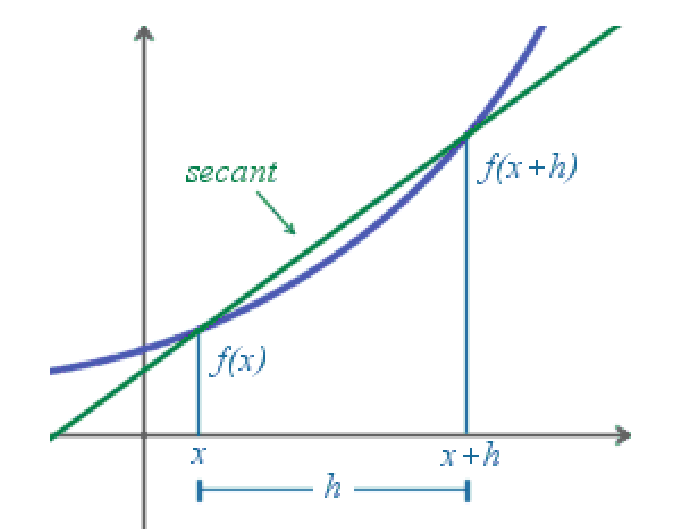
\includegraphics[scale=0.35]{img/derivadaProgresiva.png}
	\caption{Derivada progresiva}
	\label{fig:derivadaProgresiva}
\end{figure}

Calculando la pendiente de la recta secante de la figura \ref{fig:derivadaProgresiva} se obtiene una aproximación a la derivada.
\begin{align}
	m &= \dfrac{f(x+h)-f(x)}{x+h-x}\nonumber\\
		&= \dfrac{f(x+h)-f(x)}{h}\nonumber\\
	f'(x) &= \dfrac{f(x+h)-f(x)}{h}
	\label{eq:derivadaProgresiva1}
\end{align}

La expresión (\ref{eq:derivadaProgresiva1}) es una aproximación a la derivada de la función $f(x)$ 
siempre y cuando el valor de $h$ sea pequeño. Sin embargo, para una aproximación más exacta a la primera derivada se puede 
utilizar una serie de Taylor (\ref{eq:serieTaylor}).
\begin{align}
	f(x) &= \sum_{n=0}^\infty \dfrac{f^{(n)}(a)}{n!}(x-a)^n\nonumber\\
		&= f(a) + \dfrac{f'(a)}{1!}(x-a) + \dfrac{f''(a)}{2!}(x-a)^2 + \dfrac{f^{(3)}(a)}{3!}(x-a)^3 + \cdots + \dfrac{f^{(n)}(a)}{n!}(x-a)^n
	\label{eq:serieTaylor}
\end{align}


Desarrollando la serie para $f(x)$ centrada en $a=x$ y para $x=x+h$.
\begin{align*}
	f(x+h) &= f(x) + \dfrac{f'(x)}{1!}(x+h-x) + \dfrac{f''(x)}{2!}(x+h-x)^2 + \cdots + \dfrac{f^{(n)}(x)}{n!}(x+h-x)^n\\
		&= f(x) + f'(x)\cdot h + \dfrac{f''(x)}{2!}\cdot h^2 + \cdots + \dfrac{f^{(n)}(x)}{n!}\cdot h^n\\
\end{align*}
Dado que sólo nos interesa la primera derivada, se toman los primeros tres términos de la serie.
\begin{align*}
	f(x+h) &\approx f(x) + f'(x)\cdot h + \dfrac{f''(x)}{2!}\cdot h^2
\end{align*}
Despejando $f'(x)$ se obtiene la expresión (\ref{eq:derivadaProgresiva2})
\begin{definitionT}
	\begin{align}
		f'(x) &\approx \dfrac{f(x+h)-f(x)}{h} - \dfrac{f''(x)}{2!}\cdot h.
		\label{eq:derivadaProgresiva2}
	\end{align}
\end{definitionT}

\subsection{Diferencia regresiva}
Otra alternativa es aproximar la derivada de nueva cuenta con una recta secante a la función. Vease la figura \ref{fig:derivadaRegresiva}.
\begin{figure}[ht]
	\centering
	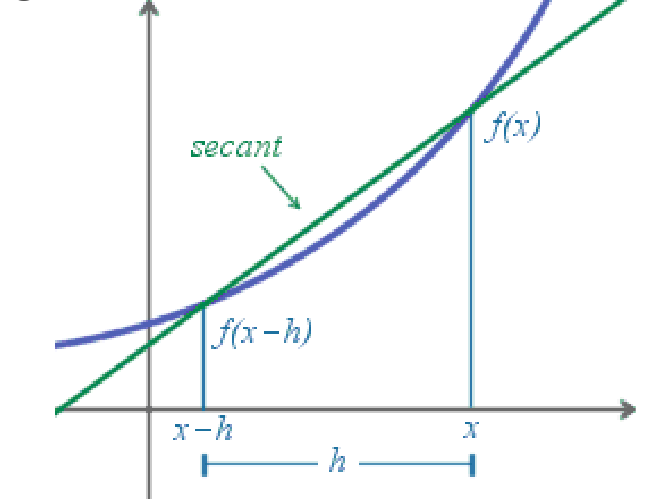
\includegraphics[scale=0.35]{img/derivadaRegresiva.png}
	\caption{Derivada regresiva}
	\label{fig:derivadaRegresiva}
\end{figure}

La diferencia sustancial en esta variante del procedimiento es que el valor diferencial $h$ se resta, en lugar de sumarse tal como el caso
anterior. Esto implica que el punto para formar la recta secante será anterior a $x$.

Calculando la pendiente de la recta secante para esta alternativa de la figura \ref{fig:derivadaRegresiva} se obtiene otra aproximación 
a la derivada.
\begin{align}
	m &= \dfrac{f(x)-f(x-h)}{x-(x-h)}\nonumber\\
	f'(x) &= \dfrac{f(x)-f(x-h)}{h}
	\label{eq:derivadaRegresiva1}
\end{align}
De nueva cuenta la expresión (\ref{eq:derivadaRegresiva1}) es una aproximación a la derivada de la función $f(x)$ 
siempre y cuando el valor de $h$ sea pequeño. Se desarrolla ahora la serie de Taylor para $f(x)$ centrada en $a=x-h$ y para $x=x$.
\begin{align*}
	f(x-h) &= f(x) + \dfrac{f'(x)}{1!}(x-h-x) + \dfrac{f''(x)}{2!}(x-h-x)^2 + \cdots + \dfrac{f^{(n)}(x)}{n!}(x-h-x)^n\\
		&= f(x) - f'(x)\cdot h + \dfrac{f''(x)}{2!}\cdot h^2 + \cdots + (-1)^n\cdot\dfrac{f^{(n)}(x)}{n!}\cdot h^n\\
\end{align*}
Dado que sólo nos interesa la primera derivada, se toman los primeros tres términos de la serie.
\begin{align*}
	f(x-h) &\approx f(x) - f'(x)\cdot h + \dfrac{f''(x)}{2!}\cdot h^2
\end{align*}
Despejando $f'(x)$  se obtiene la expresión (\ref{eq:derivadaRegresiva2})
\begin{definitionT}[Derivada Regresiva]
	\begin{equation}
		f'(x) \approx \dfrac{f(x)-f(x-h)}{h} + \dfrac{f''(x)}{2!}\cdot h.
	\label{eq:derivadaRegresiva2}
	\end{equation}
\end{definitionT}

\begin{exerciseT}{\rm
Utilice la derivada progresiva y regresiva para encontrar una aproximación a la derivada de la función $f(x) = xe^x$ en $x=2$. 
Compare los resultados obtenidos por ambos métodos.

\subsection*{Planteamiento}
Para este ejercicio se utilizará $h=0.1$. 

\subsection*{Desarrollo}

Derivación Progresiva
\begin{align*}
	f'(2) &\approx \dfrac{f(2+0.1)-f(2)}{0.1} = \dfrac{f(2.1)-f(2)}{0.1} \\
		&\approx \dfrac{2.1e^{2.1}-2e^2}{0.1}\\
		&\approx 23.7084
\end{align*}

Derivación Regresiva
\begin{align*}
	f'(2) &\approx \dfrac{f(2)-f(2-0.1)}{0.1} = \dfrac{f(2)-f(1.9)}{0.1} \\
		&\approx \dfrac{2e^2 - 1.9e^{1.9}}{0.1}\\
		&\approx 20.7491
\end{align*}
La figura \ref{fig:derivada01} muestra una comparación de las rectas obtenidas por estos cálculos, estas rectas
secante son aproximaciones a la tangente, que a su vez es la derivada de la función para $x=2$.
\begin{figure}[H]
	\centering
	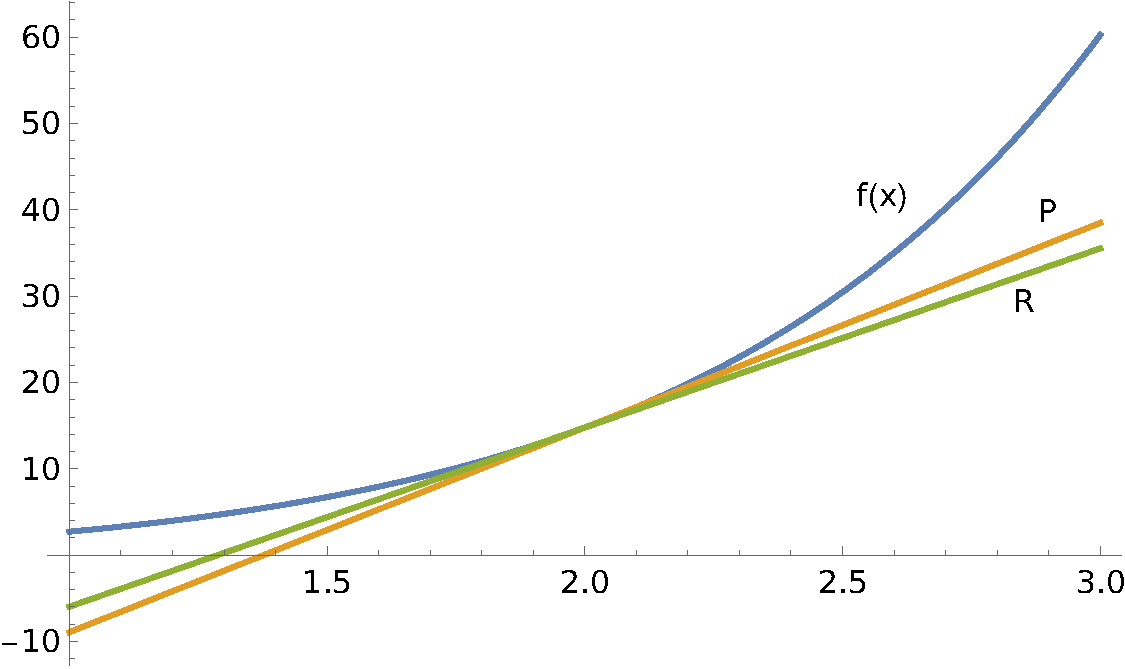
\includegraphics[scale=0.5]{img/Derivada01.pdf}
	\caption{Comparación de las primeras aproximaciones del Ejemplo \ref{ex:derivada01}}
	\label{fig:derivada01}
\end{figure}
La recta naranja (marcada con la letra P) corresponde a la obtenida por la derivación progresiva, mientras que la 
recta verde (marcada con la letra R) corresponde a la obtenida por derivación regresiva.

Es notorio que para obtener un mejor resultado en las aproximaciones se debe utilizar un valor más pequeño para $h$.
Gráficamente observaríamos que las rectas secantes se aproximan cada vez más a la tangente. La tabla \ref{table:derivada01} 
muestra los cálculos para diversos valores de $h$.

\begin{table}[H]
	\centering
	\begin{tabular}{ccc}
		\toprule
		h & D. Progresiva & D. Regresiva \\
		\midrule
		0.1 & 23.7084 & 20.7491 \\
		0.05 & 22.9217 & 21.4434 \\
		0.01 & 22.3156 & 22.02 \\
		0.005 & 22.2412 & 22.0934 \\
		0.001 & 22.182 & 22.1524 \\
		0.0001 & 22.1686 & 22.1657 \\
		0.00001 & 22.1673 & 22.167\\
		\bottomrule
	\end{tabular}
	\label{table:derivada01}
	\caption{Resultados del Ejercicio \ref{ex:derivada01}}
\end{table}
\label{ex:derivada01}
}\end{exerciseT}

\section{Fórmula de tres puntos}
\label{section:d3p}
Una estrategia distinta para obtener aproximaciones a la derivada de una función consiste en utilizar la interpolación para ello.
La idea se basa en el hecho de que un polinomio es continuo y derivable para todos los números reales. Como una ventaja adicional, 
el polinomio es fácilmente derivable. 

De esta forma la estrategia consiste en construir un polinomio de interpolación que aproxime 
a la función que se desea derivar, ahora se deriva el polinomio y se evalúa en el punto que se desea aproximar. De acuerdo al grado
del polinomio que se haya construido, la aproximación del resultado con la derivada será mejor. En términos generales se puede decir
que \textit{a mayor grado del polinomio mejor la aproximación a la derivada}.

Para la construcción del polinomio se utiliza la interpolación de Lagrange de la ecuación (\ref{eq:polinomioLagrange}). Supongamos 
que $\{x_0,x_1,\dots,x_n\}$ son $(n+1)$ números distintos en algún intervalo $I$ y que $f\in C^{n+1}(I)$. Entonces:
\[ f(x) = \sum_{k=0}^n f(x_k)L_{n,k}(x) \]
Al derivar esta expresión y evaluar $x=x_j$ se obtiene
\begin{equation}
	f'(x_j) = \sum_{k=0}^n f(x_k)L'_{n,k}(x_j)
	\label{eq:formula(n+1)Puntos} 
\end{equation}

que recibe el nombre de fórmula de $(n+1)$ puntos para aproximar $f'(x_j)$ donde $x_j$ es el valor en el que se evalúa la derivada.

En términos generales, la utilización de más puntos de evaluación en la ecuación (\ref{eq:formula(n+1)Puntos}) produce una mayor 
exactitud, aunque esto puede no ser conveniente dada la cantidad de evaluaciones funcionales y el aumento en el error de redondeo. 
Por esta razón es que se limita a formulas de tres y cinco puntos de evaluación. 

Para los tres puntos el polinomio de interpolación de Lagrange que corresponde es de segundo grado
\[ f(x) = f(x_0)L_0(x) + f(x_1)L_1(x) + f(x_2)L_2(x) \]
y su derivada es
\[ f'(x) = f(x_0)L_0'(x) + f(x_1)L_1'(x) + f(x_2)L_2'(x).\]
De esta forma, el primer término de Lagrange es
\[ L_0(x) = \dfrac{(x-x_1)(x-x_2)}{(x_0-x_1)(x_0-x_2)} \]
y su derivada con respecto a $x$ es
\[ L'_0(x) = \dfrac{2x-x_1-x_2}{(x_0-x_1)(x_0-x_2)}. \]
Para los términos de Lagrange $L_1$ y $L_2$ el resultado es muy similar, por lo que son 
\[ L'_1(x) = \dfrac{2x-x_0-x_2}{(x_1-x_0)(x_1-x_2)} \]
y 
\[ L'_2(x) = \dfrac{2x-x_0-x_1}{(x_2-x_0)(x_2-x_1)}. \]
Ahora sustituyendo la derivada de los términos de Lagrange en la ecuación \ref{eq:formula(n+1)Puntos} queda,
\begin{equation}
	f'(x_j) = f(x_0)\left[\dfrac{2x_j - x_1 - x_2}{(x_0-x_1)(x_0-x_2)}\right] + 
	f(x_1)\left[\dfrac{2x_j - x_0 - x_2}{(x_1-x_0)(x_1-x_2)}\right] 
	+ f(x_2)\left[{2x_j - x_0 - x_1\over (x_2-x_0)(x_2-x_1)}\right].
	\label{eq:formulaDerivadaTresPuntos}
\end{equation}
La ecuación (\ref{eq:formulaDerivadaTresPuntos}) es una aproximación a la derivada de $f$ evaluada en $x_j$ para tres puntos:
$x_0$, $x_1$ y $x_2$.

Ahora, si se distribuyen los puntos de forma equidistante, esto es 
\begin{align*}
	\mbox{Sea }& h\in\mathbb{R} \wedge h\not=0 \\
	x_j &= x_0\\
	x_1 &= x_0 + h \\ 
	x_2 &= x_1 + h = x_0+2h,
\end{align*}
entonces la ecuación (\ref{eq:formulaDerivadaTresPuntos}) se reduce a la expresión (\ref{eq:d3ppe}).

\begin{definitionT}[Fórmula de tres puntos - punto extremo]
	\begin{equation}
		f'(x_0) = \dfrac{1}{2h}\left[-3f(x_0)+4f(x_0+h)-f(x_0+2h)\right]
		\label{eq:d3ppe}
	\end{equation}
\end{definitionT}

Ahora, utilizando nuevamente la expresión (\ref{eq:formulaDerivadaTresPuntos}) con los tres puntos $x_0$, $x_1$ y $x_2$ 
pero acomodandolos de manera equidistante pero con $x_0$ al centro, esto es:
\begin{align*}
	\mbox{Sea }& h\in\mathbb{R} \wedge h\not=0 \\
	x_j &= x_0\\
	x_1 &= x_0 - h \\ 
	x_2 &= x_0 + h,
\end{align*}
entonces la ecuación (\ref{eq:formulaDerivadaTresPuntos}) se reduce a la expresión (\ref{eq:d3ppm}).

\begin{definitionT}[Fórmula de tres puntos - punto medio]
	\begin{equation}
		f'(x_0) = \frac{1}{2h}\left[f(x_0+h) - f(x_0-h)\right] 
		\label{eq:d3ppm}
	\end{equation}
\end{definitionT}

\section{Fórmula de cinco puntos}
Los métodos presentados en las ecuaciones (\ref{eq:d3ppe}) y (\ref{eq:d3ppm}) reciben el nombre de \textbf{fórmulas de tres 
puntos}. Así mismo, existen las llamadas \textbf{fórmulas de cinco puntos} que implican la evaluación de la función en 
dos puntos más, pero cuyo término de error tiene la forma $O(h^4)$. 

Retomando la estrategia utilizada para las fórmulas de los tres puntos, en la expresión (\ref{eq:formula(n+1)Puntos})
pero ahora se consideran cinco puntos. La expresión se reduce a
\[ f(x) = f(x_0)L_0(x) + f(x_1)L_1(x) + f(x_2)L_2(x) + f(x_3)L_3(x) + f(x_4)L_4(x) \]
y su derivada es
\begin{equation}
	f'(x_j) = f(x_0)L_0'(x) + f(x_1)L_1'(x) + f(x_2)L_2'(x) + f(x_3)L'_3(x) + f(x_4)L'_4(x).
	\label{eq:formula5puntos}
\end{equation}
De esta forma, el primer término de Lagrange es
\[ L_0(x) = \dfrac{(x-x_1)(x-x_2)(x-x_3)(x-x_4)}{(x_0-x_1)(x_0-x_2)(x_0-x_3)(x_0-x_4)} \]
y su derivada con respecto a $x$ es
\[ 
	L'_0(x) = \dfrac{(x-x_1)(x-x_2)(x-x_3)+(x-x_1)(x-x_2)(x-x_4)+(x-x_1)(x-x_3)(x-x_4)+(x-x_2)(x-x_3)(x-x_4)}
	{(x_0-x_1)(x_0-x_2)(x_0-x_3)(x_0-x_4)}. 
\]
Para los términos de Lagrange  restantes $L'_1$, $L'_2$, $L'_3$ y $L'_4$ el resultado es muy similar. Sustituyendo todos ellos
en la expresión (\ref{eq:formula5puntos}), reducir los términos se obtiene una expresión semejante a (\ref{eq:formulaDerivadaTresPuntos}).

Ahora, si se distribuyen los 5 puntos $x_0$, $x_1$, $x_2$, $x_3$ y $x_4$ de forma equidistante, y el valor $x_0$ encontrándose
en el extremo izquierdo, esto es:
\begin{align*}
	\mbox{Sea }& h\in\mathbb{R} \wedge h\not=0 \\
	x_j &= x_0\\
	x_1 &= x_0 + h \\ 
	x_2 &= x_0 + 2h \\
	x_3 &= x_0 + 3h \\
	x_4 &= x_0 + 4h
\end{align*}
entonces se reduce a la expresión (\ref{eq:d5ppe}).

\begin{definitionT}[Fórmula de cinco puntos - punto extremo]
	\begin{equation}
		f'(x_0) = \frac{1}{12h}\left[-25f(x_0) + 48f(x_0+h) - 36f(x_0+2h) + 16f(x_0+3h) - 3f(x_0+4h)\right]
		\label{eq:d5ppe}
	\end{equation}
\end{definitionT}

Si por otro lado se distribuyen los 5 puntos $x_0$, $x_1$, $x_2$, $x_3$ y $x_4$ de forma equidistante, y el valor $x_0$ encontrándose
en el centro, esto es:
\begin{align*}
	\mbox{Sea }& h\in\mathbb{R} \wedge h\not=0 \\
	x_j &= x_0\\
	x_1 &= x_0 - h \\ 
	x_2 &= x_0 - 2h \\
	x_3 &= x_0 + h \\
	x_4 &= x_0 + 2h
\end{align*}
entonces se reduce a la expresión (\ref{eq:d5ppm}).

\begin{definitionT}[Fórmula de cinco puntos - punto medio]
	\begin{equation}
		f'(x_0) = \frac{1}{12h}\left[f(x_0-2h) - 8f(x_0-h) + 8f(x_0+h) - f(x_0+2h) \right]
		\label{eq:d5ppm}
	\end{equation}
\end{definitionT}

\section{Fórmula de 3 puntos para la segunda derivada}
Si se retoma el procedimiento de la sección \ref{section:d3p} y en particular la expresión (\ref{eq:formula(n+1)Puntos}), sólo
que en esta ocasión se deriva nuevamente la expresión para obtener una segunda derivada del polinomio $f(x)$ dado por la serie 
de Taylor. Esto es:
\begin{equation}
	f''(x_j) = \sum_{k=0}^n f(x_k)L''_{n,k}(x_j)
	\label{eq:formula2d(n+1)Puntos} 
\end{equation}
Esta expresión (\ref{eq:formula2d(n+1)Puntos}) requiere a su vez de la segunda derivada de $L_0$, $L_1$ y $L_2$. Derivando estos
términos y sustituyendo se obtendría una expresión semejante a (\ref{eq:formulaDerivadaTresPuntos}). Ahora distribuyendo de 
forma equidistante los valores $x_0$, $x_1$ y $x_2$, con el valor $x_0$ en el centro, esto es:
\begin{align*}
	\mbox{Sea }& h\in\mathbb{R} \wedge h\not=0 \\
	x_j &= x_0\\
	x_1 &= x_0 - h \\ 
	x_2 &= x_0 + h,
\end{align*}
entonces la ecuación (\ref{eq:formula2d(n+1)Puntos}) se reduce a la expresión (\ref{eq:2d3ppm}).
\begin{definitionT}[Fórmula segunda derivada tres puntos - punto medio]
	\begin{equation}
		f''(x_0) = \frac{1}{h^2}\left[f(x_0-h) - 2f(x_0) + f(x_0+h)\right] 
		\label{eq:2d3ppm}
	\end{equation}
\end{definitionT}


\begin{exerciseT}
	Dada la función $f(x) = xe^x$, 
		\begin{enumerate}[a)]
			\item Utilice las fórmulas de los 3 y 5 puntos para encontrar aproximaciones a la primera derivada de 
				la función $f(x)$ en $x=2$. 
			\item ¿Qué fórmula permite encontrar un mejor resultado?, ¿porque?
			\item Utilice también la fórmula de los 3 puntos para obtener una aproximación a la segunda derivada de $f(x)$ en $x=2$.
		\end{enumerate}	
	
\end{exerciseT}


\section{Integración numérica: Método del trapecio}
\section{Integración numérica: Métodos de Simpson}
\section{Integración numérica: Integración de Romberg}
\section{Integración numérica: Método de cuadratura gaussiana}
\section{Integración múltiple}
\section{Aplicaciones}




%----------------------------------------------------------------------------------------
%	PART
%----------------------------------------------------------------------------------------

%\part{Parte 2}

%----------------------------------------------------------------------------------------
%	CHAPTER 7
%----------------------------------------------------------------------------------------

\chapter{Plataformas para el modelado computacional}

\section{Herramientas tradicionales de programación}

\subsection{Fortran}

\subsection{C}

\subsection{C++}

\section{Microsoft Excel}

\section{Wolfram Mathematica}

\section{Matlab}

\section{Otras plataformas}


%----------------------------------------------------------------------------------------
%	BIBLIOGRAPHY
%----------------------------------------------------------------------------------------

\chapter*{Bibliography}
\addcontentsline{toc}{chapter}{\textcolor{ocre}{Bibliography}}

%------------------------------------------------

\section*{Articles}
\addcontentsline{toc}{section}{Articles}
\printbibliography[heading=bibempty,type=article]

%------------------------------------------------

\section*{Books}
\addcontentsline{toc}{section}{Books}
\printbibliography[heading=bibempty,type=book]


\end{document}
